\documentclass[12pt]{book}
\usepackage[hidelinks]{hyperref}
\usepackage{graphicx}
\usepackage{listings}
\usepackage{xcolor}
\usepackage{lscape}
\usepackage{url}
\usepackage{tikz,mathpazo}
\usetikzlibrary{shapes.geometric, arrows}
%Define listing environment and properties
\lstset { breaklines=true , breakindent=0pt , language={Python} , keywordstyle=\color {blue} , frame=shadowbox}

\tikzstyle{startstop} = [rectangle, rounded corners, minimum width=3cm, minimum height=1cm,align=center, draw=black, fill=red!30]
\tikzstyle{io} = [trapezium, trapezium left angle=70, trapezium right angle=110, minimum width=3cm, minimum height=1cm, align=center, draw=black, fill=blue!30]
\tikzstyle{process0} = [rectangle, minimum width=3cm, minimum height=1cm,align=center, draw=black, fill=magenta!30]
\tikzstyle{process1} = [rectangle, minimum width=3cm, minimum height=1cm,align=center, draw=black, fill=orange!30]
\tikzstyle{process2} = [rectangle, minimum width=4.8cm, minimum height=1cm,align=left, draw=black, fill=yellow!30]
\tikzstyle{decision} = [diamond, minimum width=3cm, minimum height=1cm,align=center, draw=black, fill=green!30]
\tikzstyle{arrow} = [thick,->]

\graphicspath{{./figs/}}

\begin{document}
%\title{\Huge\textbf{MATSDP} \\
%\large The materials simulation and data processing toolkit \\
%\large version 0.1.2}
%\vspace{1.5cm}
%\vfill
%\author{Dianwu Wang \\ \href{mailto:dianwuwang@163.com}{dianwuwang@163.com}}
%\vspace{0.8cm}
%\date{September 11, 2019}
%\large 
%\maketitle

\begin{titlepage}
\begin{center}
\vspace*{1cm}

\Huge
\textbf{MATSDP}

\vspace{0.5cm}
\LARGE The materials simulation and data processing toolkit
\vspace{1.5cm}

\vfill

%\small Dianwu Wang \\
%\small dianwuwang@163.com \\
\vspace{0.8cm}

\small version 0.2.1\\
\small Dec. 9, 2020

\end{center}
\end{titlepage}

\tableofcontents

\chapter{Introduction}
MATSDP is a materials simulation and data processing toolkit. The Vienna ab-initio simulation package (VASP) and the Three-dimensional atom probe tomography (APT) analyzing and data processing tools are included. 

\section{Functions}

VASP analyzing and data processing tools:
\begin{itemize}
\item Build model by atom substitution or atom selection based on a POSCAR file
\item Read VASP inputs and outputs
\item Plot model in the POSCAR/CONTCAR (also support color mapping of atom properties).
\item Plot DOS (PDOS, LDOS, TDOS), band structure (including fat band).
\item Calculate the nearest neighbor information.
\item Perform simple common neighbor analysis
\item Calculate structural energy.
\item Write atom force information into the POSCAR file.
\end{itemize}

APT postprocessing tools:
\begin{itemize}
\item Read the concentration profile *.csv file
\item Plot the concentration profile
\end{itemize}

DVM tools:
\begin{itemize}
\item Read the *.input, *.incar, *.otput files
\item Write the *.input, *.incar, IND.DAT files
\item Write the interatomic energy (IE) files (including the IEs of the first nearest neighbor atoms)
\item The *.incar file can also be prepared by atom selection from the vasp\_build function in the vasp module 
\end{itemize}

Others tools:
\begin{itemize}
\item file format conversion
\item project manager
\end{itemize}

%\begin{tikzpicture}[line width=3pt, node distance=4cm]
%\def \smbwd{2cm}
%\node (vasp) [startstop] {vasp};
%\node (vasp_read) [process1, below of=vasp,xshift=-5.3cm] {vasp\_read};
%\node (vasp_build) [process1, right of=vasp_read] {vasp\_build};
%\node (vasp_plot) [process1, right of=vasp_build] {vasp\_plot};
%\node (vasp_analyze) [process1, right of=vasp_plot] {vasp\_analyze};
%
%\node (vasp_read_sub) [process2, below of=vasp_read] {read\_incar\\read\_poscar\\read\_outcar\\read\_doscar};
%\node (vasp_build_sub) [process2, below of=vasp_build] {substitution\\rep\_elmt};
%\node (vasp_plot_sub) [process2, below of=vasp_plot] {plot\_dos\\plot\_poscar\\plot\_poscar \\ \_for\_workdir};
%\node (vasp_analyze_sub) [process2, below of=vasp_analyze] {nn\_map\\estruct\\overlap\_peak \\ \_analyzer};
%
%\draw[arrow] (vasp) -- (vasp_read);
%\draw[arrow] (vasp) -- (vasp_build);
%\draw[arrow] (vasp) -- (vasp_plot);
%\draw[arrow] (vasp) -- (vasp_analyze);
%
%\draw[arrow] (vasp_read) -- (vasp_read_sub);
%\draw[arrow] (vasp_build) -- (vasp_build_sub);
%\draw[arrow] (vasp_plot) -- (vasp_plot_sub);
%\draw[arrow] (vasp_analyze) -- (vasp_analyze_sub);
%\end{tikzpicture}

The matsdp package contains the vasp module, the apt module and the dvm module as shown in Figure \ref{fig:matsdp_main_structure}. The structures of the vasp module, the apt module and the dvm module are shown in Figure \ref{fig:vasp_module}, Figure \ref{fig:apt_module}, and Figure \ref{fig:dvm_module}.

\begin{figure}[htbp]
\centering
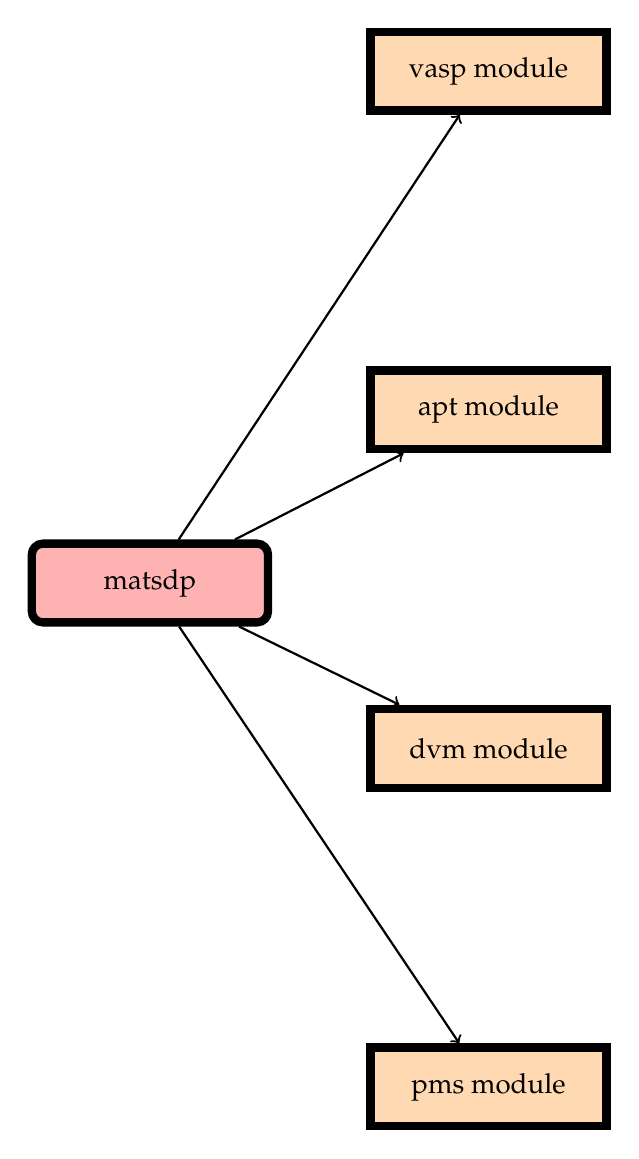
\begin{tikzpicture}[line width=3pt, node distance=4.3cm]
\def \smbwd{2cm}
\node (matsdp) [startstop] {matsdp};
\node (vasp) [process1, right of=matsdp,yshift=6.5cm] {vasp module};
\node (apt) [process1, below of=vasp] {apt module};
\node (dvm) [process1, below of=apt] {dvm module};
\node (pms) [process1, below of=dvm] {pms module};

\draw[arrow] (matsdp) -- (vasp);
\draw[arrow] (matsdp) -- (apt);
\draw[arrow] (matsdp) -- (dvm);
\draw[arrow] (matsdp) -- (pms);
\end{tikzpicture}
\caption{\label{fig:matsdp_main_structure} subpackages of the matsdp program.}
\end{figure}

\begin{figure}[htbp]
\centering
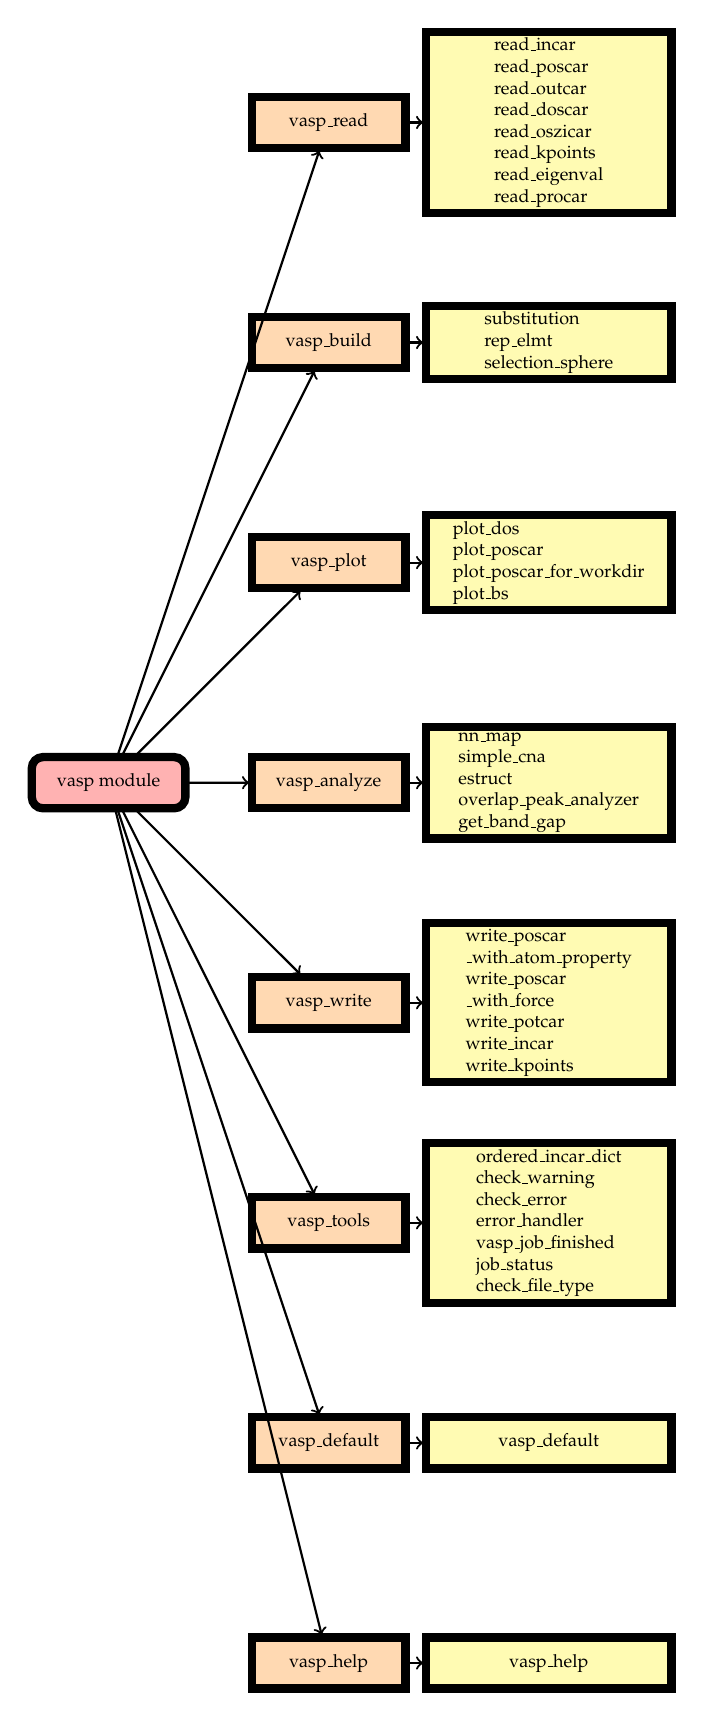
\begin{tikzpicture}[line width=3pt, node distance=4.3cm]
%\tikzstyle{every node}=[font=\small,scale=0.9]
\tikzstyle{every node}=[scale=0.65]
\def \smbwd{2cm}
\node (vasp) [startstop] {vasp module};
\node (vasp_read) [process1, right of=vasp,yshift=12.90cm] {vasp\_read};
\node (vasp_build) [process1, below of=vasp_read] {vasp\_build};
\node (vasp_plot) [process1, below of=vasp_build] {vasp\_plot};
\node (vasp_analyze) [process1, below of=vasp_plot] {vasp\_analyze};
\node (vasp_write) [process1, below of=vasp_analyze] {vasp\_write};
\node (vasp_tools) [process1, below of=vasp_write] {vasp\_tools};
\node (vasp_default) [process1, below of=vasp_tools] {vasp\_default};
\node (vasp_help) [process1, below of=vasp_default] {vasp\_help};

\node (vasp_read_sub) [process2, right of=vasp_read] {read\_incar\\read\_poscar\\read\_outcar\\read\_doscar\\read\_oszicar\\read\_kpoints\\read\_eigenval\\read\_procar};
\node (vasp_build_sub) [process2, right of=vasp_build] {substitution\\rep\_elmt\\selection\_sphere};
\node (vasp_plot_sub) [process2, right of=vasp_plot] {plot\_dos\\plot\_poscar\\plot\_poscar\_for\_workdir\\plot\_bs};
\node (vasp_analyze_sub) [process2, right of=vasp_analyze] {nn\_map\\simple\_cna\\estruct\\overlap\_peak\_analyzer\\get\_band\_gap};
\node (vasp_write_sub) [process2, right of=vasp_write] {write\_poscar\\ \_with\_atom\_property\\write\_poscar\\ \_with\_force\\write\_potcar\\write\_incar\\write\_kpoints};
\node (vasp_tools_sub) [process2, right of=vasp_tools] {ordered\_incar\_dict\\check\_warning\\check\_error\\error\_handler\\vasp\_job\_finished\\job\_status\\check\_file\_type};
\node (vasp_default_sub) [process2, right of=vasp_default] {vasp\_default};
\node (vasp_help_sub) [process2, right of=vasp_help] {vasp\_help};

\draw[arrow] (vasp) -- (vasp_read);
\draw[arrow] (vasp) -- (vasp_build);
\draw[arrow] (vasp) -- (vasp_plot);
\draw[arrow] (vasp) -- (vasp_analyze);
\draw[arrow] (vasp) -- (vasp_write);
\draw[arrow] (vasp) -- (vasp_tools);
\draw[arrow] (vasp) -- (vasp_default);
\draw[arrow] (vasp) -- (vasp_help);

\draw[arrow] (vasp_read) -- (vasp_read_sub);
\draw[arrow] (vasp_build) -- (vasp_build_sub);
\draw[arrow] (vasp_plot) -- (vasp_plot_sub);
\draw[arrow] (vasp_analyze) -- (vasp_analyze_sub);
\draw[arrow] (vasp_write) -- (vasp_write_sub);
\draw[arrow] (vasp_tools) -- (vasp_tools_sub);
\draw[arrow] (vasp_default) -- (vasp_default_sub);
\draw[arrow] (vasp_help) -- (vasp_help_sub);
\end{tikzpicture}
\caption{\label{fig:vasp_module} vasp module.}
\end{figure}

\begin{figure}[htbp]
\centering
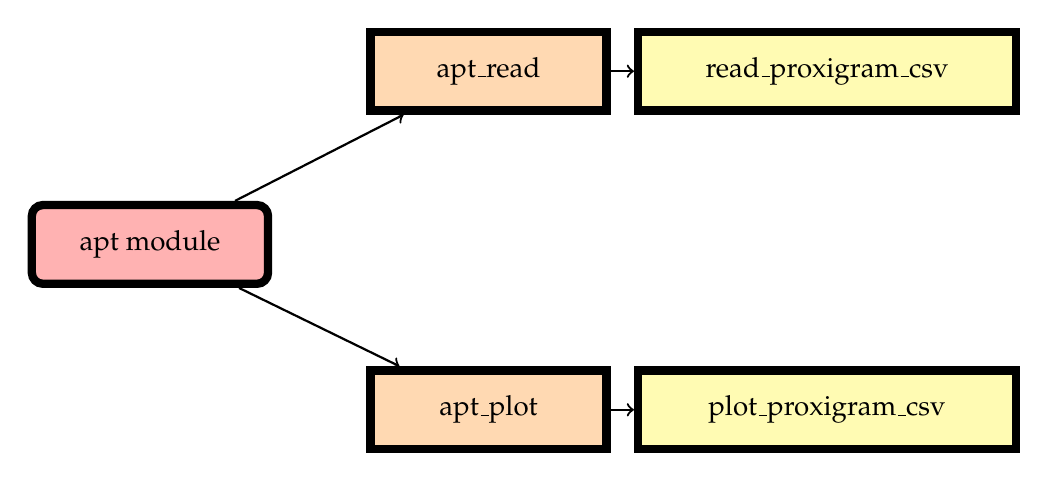
\begin{tikzpicture}[line width=3pt, node distance=4.3cm]
\def \smbwd{2cm}
\node (apt) [startstop] {apt module};
\node (apt_read) [process1, right of=apt,yshift=2.2cm] {apt\_read};
\node (apt_plot) [process1, below of=apt_read] {apt\_plot};

\node (apt_read_sub) [process2, right of=apt_read] {read\_proxigram\_csv};
\node (apt_plot_sub) [process2, right of=apt_plot] {plot\_proxigram\_csv};

\draw[arrow] (apt) -- (apt_read);
\draw[arrow] (apt) -- (apt_plot);


\draw[arrow] (apt_read) -- (apt_read_sub);
\draw[arrow] (apt_plot) -- (apt_plot_sub);
\end{tikzpicture}
\caption{\label{fig:apt_module} apt module.}
\end{figure}

\begin{figure}[htbp]
\centering
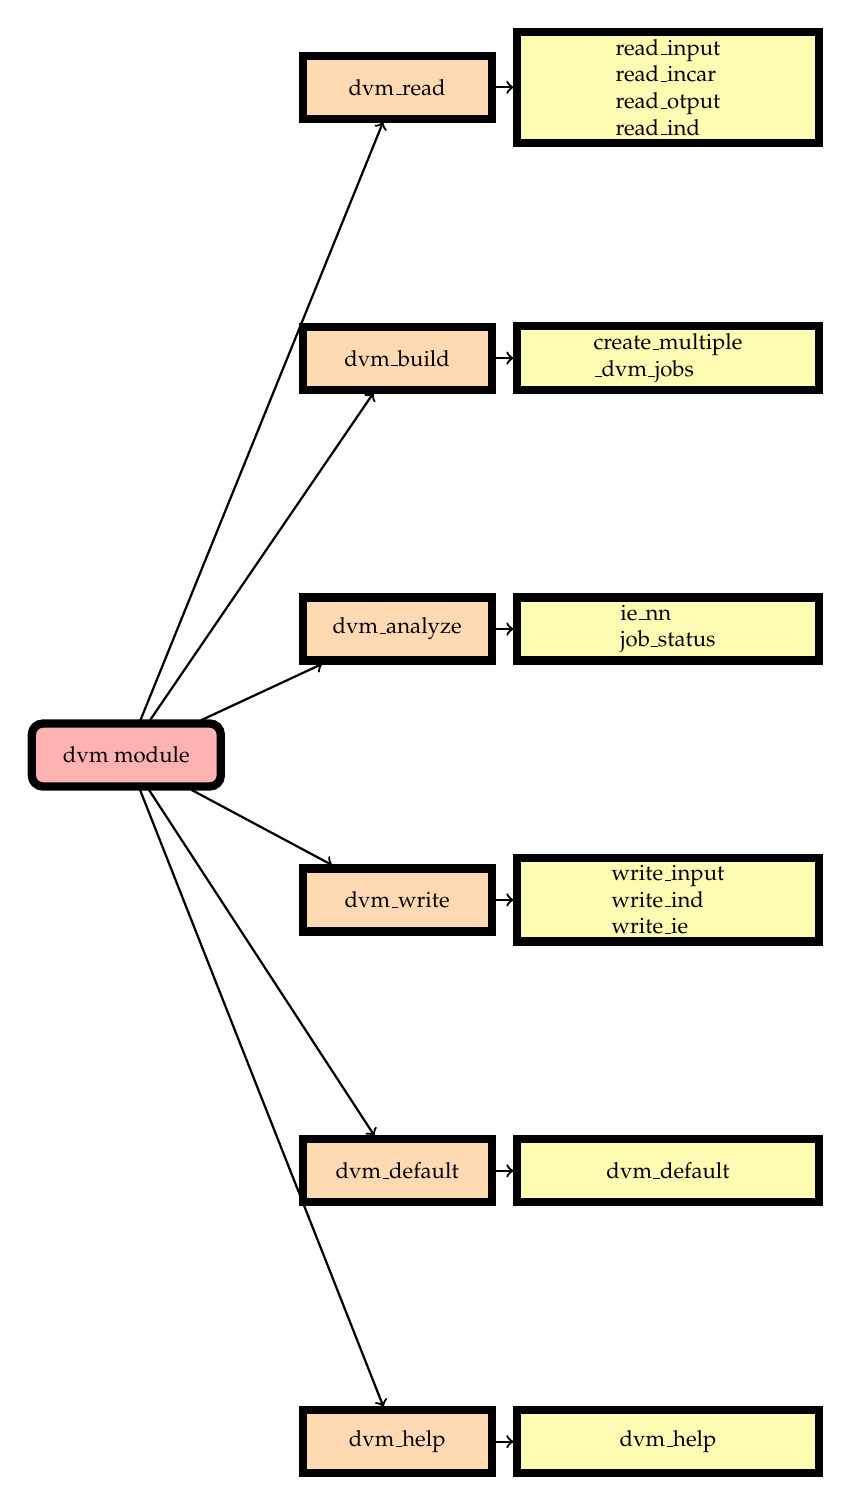
\begin{tikzpicture}[line width=3pt, node distance=4.3cm]
\tikzstyle{every node}=[scale=0.8]
\def \smbwd{2cm}
\node (dvm) [startstop] {dvm module};
\node (dvm_read) [process1, right of=dvm,yshift=10.60cm] {dvm\_read};
\node (dvm_build) [process1, below of=dvm_read] {dvm\_build};
\node (dvm_analyze) [process1, below of=dvm_build] {dvm\_analyze};
\node (dvm_write) [process1, below of=dvm_analyze] {dvm\_write};
\node (dvm_default) [process1, below of=dvm_write] {dvm\_default};
\node (dvm_help) [process1, below of=dvm_default] {dvm\_help};

\node (dvm_read_sub) [process2, right of=dvm_read] {read\_input\\read\_incar\\read\_otput\\read\_ind};
\node (dvm_build_sub) [process2, right of=dvm_build] {create\_multiple\\\_dvm\_jobs};
\node (dvm_analyze_sub) [process2, right of=dvm_analyze] {ie\_nn\\job\_status};
\node (dvm_write_sub) [process2, right of=dvm_write] {write\_input\\write\_ind\\write\_ie};
\node (dvm_default_sub) [process2, right of=dvm_default] {dvm\_default};
\node (dvm_help_sub) [process2, right of=dvm_help] {dvm\_help};

\draw[arrow] (dvm) -- (dvm_read);
\draw[arrow] (dvm) -- (dvm_build);
\draw[arrow] (dvm) -- (dvm_analyze);
\draw[arrow] (dvm) -- (dvm_write);
\draw[arrow] (dvm) -- (dvm_default);
\draw[arrow] (dvm) -- (dvm_help);

\draw[arrow] (dvm_read) -- (dvm_read_sub);
\draw[arrow] (dvm_build) -- (dvm_build_sub);
\draw[arrow] (dvm_analyze) -- (dvm_analyze_sub);
\draw[arrow] (dvm_write) -- (dvm_write_sub);
\draw[arrow] (dvm_default) -- (dvm_default_sub);
\draw[arrow] (dvm_help) -- (dvm_help_sub);
\end{tikzpicture}
\caption{\label{fig:dvm_module} dvm module.}
\end{figure}

%\begin{tikzpicture}[line width=3pt, node distance=4.3cm]
%\def \smbwd{2cm}
%\node (matsdp) [startstop] {matsdp};
%
%\node (vasp) [process0,right of=matsdp,yshift=5.9cm] {vasp module};
%
%\node (vasp_read) [process1, right of=vasp,yshift=6.45cm] {vasp\_read};
%\node (vasp_build) [process1, below of=vasp_read] {vasp\_build};
%\node (vasp_plot) [process1, below of=vasp_build] {vasp\_plot};
%\node (vasp_analyze) [process1, below of=vasp_plot] {vasp\_analyze};
%
%\node (vasp_read_sub) [process2, right of=vasp_read] {read\_incar\\read\_poscar\\read\_outcar\\read\_doscar};
%\node (vasp_build_sub) [process2, right of=vasp_build] {substitution\\rep\_elmt};
%\node (vasp_plot_sub) [process2, right of=vasp_plot] {plot\_dos\\plot\_poscar\\plot\_poscar\_for\_workdir};
%\node (vasp_analyze_sub) [process2, right of=vasp_analyze] {nn\_map\\estruct\\overlap\_peak\_analyzer};
%
%\node (apt) [process0,below of=vasp,yshift=-7.45cm] {apt module};
%
%\node (apt_read) [process1, right of=apt,yshift=2.1cm] {apt\_read};
%\node (apt_plot) [process1, below of=apt_read] {apt\_plot};
%
%\node (apt_read_sub) [process2, right of=apt_read] {read\_proxigram\_csv};
%\node (apt_plot_sub) [process2, right of=apt_plot] {plot\_proxigram\_csv};
%
%
%\draw[arrow] (matsdp) -- (vasp);
%
%\draw[arrow] (vasp) -- (vasp_read);
%\draw[arrow] (vasp) -- (vasp_build);
%\draw[arrow] (vasp) -- (vasp_plot);
%\draw[arrow] (vasp) -- (vasp_analyze);
%
%\draw[arrow] (vasp_read) -- (vasp_read_sub);
%\draw[arrow] (vasp_build) -- (vasp_build_sub);
%\draw[arrow] (vasp_plot) -- (vasp_plot_sub);
%\draw[arrow] (vasp_analyze) -- (vasp_analyze_sub);
%
%\draw[arrow] (matsdp) -- (apt);
%
%\draw[arrow] (apt) -- (apt_read);
%\draw[arrow] (apt) -- (apt_plot);

%\draw[arrow] (apt_read) -- (apt_read_sub);
%\draw[arrow] (apt_plot) -- (apt_plot_sub);
%\end{tikzpicture}

%\newpage
%\section{File structure}
%
%\begin{lstlisting}[numbers=none]
%matsdp/
%|-- __init__.py
%|-- convert.py
%|-- default_params.py
%|-- funcs.py
%|-- periodic_table.py
%|-- vasp/
%|    |-- __init__.py
%|    |-- vasp_analyze.py
%|    |-- vasp_build.py
%|    |-- vasp_plot.py
%|    |-- vasp_read.py
%|    |-- vasp_write.py
%|    |-- vasp_default.py
%|    |-- vasp_help.py
%|-- apt/
%|    |-- __init__.py
%|    |-- apt_plot.py
%|    |-- apt_read.py
%|-- dvm/
%|    |-- __init__.py
%|    |-- dvm_analyze.py
%|    |-- dvm_build.py
%|    |-- dvm_read.py
%|    |-- dvm_write.py
%|    |-- dvm_default.py
%|    |-- dvm_help.py
%\end{lstlisting}
%%|-- tests/
%%|    |-- __init__.py
%%|    |-- runtests.py
%%|    |-- a.py
%%|    |-- b.py
%%|    |-- data/
%%|    |   |-- INCAR
%%|    |   |-- OUTCAR
%%|    |   |-- DOSCAR

\section{Requirements}
\begin{itemize}
\item numpy
\item scipy
\item scikit-learn
\item matplotlib
\end{itemize}

\section{Installation}
For the Python users, the package can be retrieved by the following command. 
\begin{lstlisting}
pip install matsdp
\end{lstlisting}

For the GUI users, please run the matsdp\_gui.exe directly.

\section{Usage}
\subsection{Running with Python environment}
After installing the matsdp package, the program can be used by importing the modules and call the related functions.
\subsection{Running Graphical User Interface (GUI) application}
The program provides a graphical user interface (matsdp\_gui.exe). The GUI is shown in the Figure \ref{fig:GUI_Main}:

\begin{figure}[htbp]
\centering
\includegraphics[width=0.9\textwidth]{gui_matsdp.pdf}
\caption{GUI for the main program}
\label{fig:GUI_Main}
\end{figure}

\section{Notes}

Note that for the module that requires POSCAR/CONTCAR, OUTCAR and DOSCAR files, these files need to be in the same folder.

The following sections will introduce the settings of the parameters in the GUI. 

%%%%%%%%%%%%%%%%
%VASP
%%%%%%%%%%%%%%%%
\chapter{Subpackage: vasp}

Modules that may be imported before using the vasp package
\begin{itemize}
\item from matsdp.vasp import vasp\_read
\item from matsdp.vasp import vasp\_build
\item from matsdp.vasp import vasp\_plot
\item from matsdp.vasp import vasp\_analyze
\item from matsdp.vasp import vasp\_write
\item from matsdp.vasp import vasp\_tools
\item from matsdp.vasp import vasp\_default
\item from matsdp.vasp import vasp\_help
\end{itemize}

%%%%%%%%%%%%%%
%vasp\_build
%%%%%%%%%%%%%%
\section{vasp\_build module}
\subsection{vasp\_build.substitution}
\subsubsection{Descriptions}
Building models by substitution of atoms
\subsubsection{Syntax}
\begin{lstlisting}
from matsdp.vasp import vasp_build
vasp_build.substitution(
    substitution_list_file = './example/vasp/example/vasp.subst',
    poscar_file_path = './example/vasp/POSCAR_NoDope',
    )
\end{lstlisting}
\subsubsection{Arguments}
\begin{itemize}
\item substitution\_list\_file: String format. It specifies the directory of the .subst file (substitution list file)
\item poscar\_file\_path: String format. The directory of the POSCAR file which is to be subsituted. It can either be full path or relative path.
\end{itemize}

\subsubsection{.subst file}

Descriptions
\begin{itemize}
\item The .subst file (substitution list file) is required and should consists of system entries.
\item A system corresponds to a specific model configuration.
\item System entries specifies how atoms are substituted in different systems.
\item A system entry is a block of successive lines without line breaks.
\item Each system entries must be separated by blank lines.
\end{itemize}

File formats. A typical system entry has the following format:
\begin{lstlisting}
n_subst
elment_name_to_be_substituted new_element_name
elment_name_to_be_substituted new_element_name
...
(n_subst lines of elment_name_to_be_substituted elment_subindx new_element_name)
\end{lstlisting}
where,
elment\_name\_to\_be\_substituted is he name of the element which is to be substituted.
new\_element\_name is the name of the new element which take the place of the substituted atom. If new\_element\_name = Va, then a vacancy is added.
As shown above, each system should start with a line which specifies a number: n\_subst.
n\_subst is the number of atoms to be substituted in the system.
Then each of the following n\_subst lines specifies the element(s) to be substituted and the element(s) which take its/their place(s).

A specific example .subst file is as follow:
\begin{lstlisting}
1
Ni244 W

2
Ni244 Re
Al12 Re

...
\end{lstlisting}

\subsubsection{GUI}
\begin{figure}[htbp]
\centering
\includegraphics[width=0.9\textwidth]{gui_substitution.pdf}
\caption{GUI for Substitution}
\label{fig:GUI_Substitution}
\end{figure}

\subsubsection{Outputs}
Outputs: The final system name is L(line\_number)\_composition\_D(duplicate)

\subsection{vasp\_build.selection\_sphere}
\subsubsection{Descriptions}
Building models by selection of atoms. The atoms within a sphere will be selected.
\subsubsection{Syntax}
\begin{lstlisting}
from matsdp.vasp import vasp_build
vasp_build.selection_sphere(
    poscar_file_path = './tests/vasp/CONTCAR',
    origin_atom_name = 'Re1',
    radius = 7,
    include_mirror_atoms = False,
    output_file_name = 'example'
    )
\end{lstlisting}
\subsubsection{Arguments}
\begin{itemize}
\item poscar\_file\_path: String format. The directory of the POSCAR file. It can either be full path or relative path.
\item origin\_atom\_name: String type. It defines the origin atom of the sphere
\item radius: Float type. The atoms within a distance ``radius'' from the original atom are selected (units in Angstroms);
\item include\_mirror\_atoms: Logical value. Whether to include the mirror atoms or not;
\item output\_file\_name: user-defined output file name.
\end{itemize}

\subsubsection{GUI}
\begin{figure}[htbp]
\centering
\includegraphics[width=0.9\textwidth]{gui_selection_sphere.pdf}
\caption{GUI for selection\_sphere}
\label{fig:GUI_selection_sphere}
\end{figure}

\subsubsection{Outputs}
Outputs: *.vasp, *.xyz, and *.incar files. The *.incar file can be used as the input file for the DVM program.

%%%%%%%%%%%%%
%vasp\_plot
%%%%%%%%%%%%%
\section{vasp\_plot module}
\subsection{vasp\_plot.plot\_poscar}
\subsubsection{Descriptions}
\begin{itemize}
\item Visualization of POSCAR model. Euler angles are used to rotate the view of the model.
\item Viewer direction is in x direction. The original orientation: x direction is perpendicular to the paper, z direction is in the paper and point to upper direction
\item Reference for Eulerian angles: Herbert Goldstein, Charles P. Poole Jr. and John L. Safko, Classical Mechanics (3rd Edition). Goldstein Poole \& Safko, 2001.
\item This module can also show the atom properties by color mapping. The POSCAR file with additional data columns used to save the data of the atom properties.
\end{itemize}

\subsubsection{Syntax}
\begin{lstlisting}
from matsdp.vasp import vasp_plot
vasp_plot.plot_poscar(
    poscar_file_path = './example/vasp/POSCAR',
    euler_angle_type = 'zyz',
    phi = -3,
    theta = 4,
    psi = 0,
    elmt_color = {'Ni':'red','Re':'blue'},
    draw_mirror_atom = True,
    box_on = True,
    axis_indicator =True,
    plot_cell_basis_vector_label = True,
    plot_atom_label = None,
    fig_format = 'png',
    fig_dpi = 100,
    draw_colormap = False,
    colormap_column_indx = 1,
    colormap_vmin = None,
    colormap_vmax = None,
    vmin_color = 'blue',
    vmax_color = 'red',
    colorbar_alignment = 'vertical'
	)
\end{lstlisting}

\subsubsection{Arguments}
\begin{itemize}
\item poscar\_file\_path: String format. Directory of the POSCAR file which you want to plot
\item euler\_angle\_type: string of length 3. It specify the type of rotations based on Eulerian angles. Choices are 'zyz', 'zxz', 'zyx', etc.. Usually the 'zyz' type is used.

            'zyz' : proper Euler angle, y-convention. Perform consecutive rotations at axes counter-clockwisely. z-y-z rotation.
                    First rotate the z axes of atoms by an angle phi, then rotate the intermediate y axis of atoms by an angle theta, finally rotate the final z axis of atoms by an angle psi

            'zxz' : proper Euler angle, x-convention. Perform consecutive rotations at axes counter-clockwisely. z-x-z rotation.
                    First rotate the z axes of atoms by an angle phi, then rotate the intermediate x axis of atoms by an angle theta, finally rotate the final z axis of atoms by an angle psi

            'zyx' : Tait-Bryan angles. z-y-x rotation. Perform consecutive rotations at axes counter-clockwisely. z-y-x rotation.
                    First rotate the z axes of atoms by an angle phi, then rotate the intermediate y axis of atoms by an angle theta, finally rotate the final x axis of atoms by an angle psi

\item phi, theta, psi: float formats. The first, second, and third rotation Eulerian angles, units in degrees.
\item elmt\_color: dictionary formats. this dictionary sepcifies the color for each element. For example elmt\_color = \{'Ni':'black','Al':'magenta'\}
\item draw\_mirror\_atom: Logical value. Whether to plot the mirror atoms at the periodic boundary
\item box\_on: Logical value. Whether to plot the box or not
\item axis\_indicator: Logic value. Whether to plot the axis indicator
\item plot\_cell\_basis\_vector\_label: Logical value. Whether to plot the cell basis vector labels( i.e., to label the three basis vectors of the cell as a, b, and c)
\item plot\_atom\_label: String value. values: ``atom\_name'', ``atom\_index'', ``atom\_species'', ``fix\_info'', ``position\_direct'', ``position\_cartesian', ``added\_atom\_data'' or None/``None''. It plots atom label to each atom
\item fig\_format: String format. fig\_format is a string that defines output figure format. Supported fig\_format: 'png', 'eps', 'pdf', 'tif', 'tiff', 'jpg', 'jpeg', 'svg', 'svgz', 'pgf', 'ps', 'raw', 'rgba'
\item fig\_dpi: float format. The DPI for non-vector graphics.
\item draw\_colormap: Logical value. If true, the color mapping of atom properties will be Performed. Default: False.
\item colormap\_column\_indx: Integer value. Define which column of the atom property columns will be color mapped. Default: 1.
\item colormap\_vmin: Float value. Define the minimum value of the color map. If colormap\_vmin=None, the minimum value of the original data will be used. Default: None.
\item colormap\_vmax: Float value. Define the maximum value of the color map. If colormap\_vmax=None, the maximum value of the original data will be used. Default: None.
\item vmin\_color = 'blue': String type. Define the color for the smallest value of the atom properties in the color map. Default: 'blue'.
\item vmax\_color = 'red': String type. Define the color for the largest value of the atom properties in the color map. Default: 'red'.
\item colorbar\_alignment: String type. Defines the alignment of the color bar in the figure of the color map. The value can be either 'vertical' or 'horizontal'. Default: 'vertical'.
\end{itemize}

\subsubsection{GUI}
The GUI of the plot\_poscar module is shown in the Figure \ref{fig:gui_plot_poscar} 
\begin{figure}[htbp]
\centering
\includegraphics[width=0.9\textwidth]{gui_plot_poscar.pdf}
\caption{GUI for matsdp.vasp.vasp\_plot.plot\_poscar}
\label{fig:gui_plot_poscar}
\end{figure}

\subsubsection{Outputs}
Figures of POSCAR models.

\subsubsection{Examples}

The examples are shown in the Figure \ref{fig:outputs_plot_poscar1}, Figure \ref{fig:outputs_plot_poscar2}, Figure \ref{fig:outputs_colormapping1} and Figure \ref{fig:outputs_colormapping2}.

\begin{figure}[htbp]
\centering
\includegraphics[width=0.7\textwidth]{outputs_plot_poscar1.pdf}
\caption{Result of the plot\_poscar module. The atom label is added.}
\label{fig:outputs_plot_poscar1}
\end{figure}

\begin{figure}[htbp]
\centering
\includegraphics[width=0.7\textwidth]{outputs_plot_poscar2.pdf}
\caption{Result of the plot\_poscar module. The atom label is removed.}
\label{fig:outputs_plot_poscar2}
\end{figure}

\begin{figure}[htbp]
\centering
\includegraphics[width=0.7\textwidth]{outputs_colormapping1.pdf}
\caption{Result of the plot\_poscar module: color mapping of atom properties. The color bar is vertically aligned.}
\label{fig:outputs_colormapping1}
\end{figure}

\begin{figure}[htbp]
\centering
\includegraphics[width=0.7\textwidth]{outputs_colormapping2.pdf}
\caption{Result of the plot\_poscar module: color mapping of atom properties. The color bar is horizontally aligned.}
\label{fig:outputs_colormapping2}
\end{figure}

\newpage

\subsection{vasp\_plot.plot\_poscar\_for\_workdir}
\subsubsection{Descriptions}
\begin{itemize}
\item Visualization of POSCARs. 
\item The mother folder needs to be specified which contains the folders with POSCARs
\item Euler angles are used to rotate the view of the model
\item This module can also show the atom properties by color mapping. The POSCAR file with additional data columns used to save the data of the atom properties.
\end{itemize}
\subsubsection{Syntax}
\begin{lstlisting}
from matsdp.vasp import vasp_plot
vasp_plot.plot_poscar_for_workdir(
    workdir = './tests/vasp/',
    euler_angle_type = 'zyx',
    phi = -3,
    theta = 4,
    psi = 0,
    elmt_color = None,
    draw_mirror_atom = True,
    box_on = True,
    axis_indicator =True,
    plot_cell_basis_vector_label = True,
    plot_atom_label = None,
    poscar_or_contcar = 'POSCAR',
    fig_format = 'png',
    fig_dpi = 100,
    draw_colormap = False,
    colormap_column_indx = 1,
    colormap_vmin = None,
    colormap_vmax = None,
    vmin_color = 'blue',
    vmax_color = 'red',
    colorbar_alignment = 'vertical'
    )
\end{lstlisting}

\subsubsection{Arguments}

\begin{itemize}
\item workdir: String format. The mother folder which contains the folders with POSCARs
\item euler\_angle\_type: string of length 3. It specify the type of rotations based on Eulerian angles. Choices are 'zyz', 'zxz', 'zyx', etc.. Usually the 'zyz' type is used.

            'zyz' : proper Euler angle, y-convention. Perform consecutive rotations at axes counter-clockwisely. z-y-z rotation.
                    First rotate the z axes of atoms by an angle phi, then rotate the intermediate y axis of atoms by an angle theta, finally rotate the final z axis of atoms by an angle psi

            'zxz' : proper Euler angle, x-convention. Perform consecutive rotations at axes counter-clockwisely. z-x-z rotation.
                    First rotate the z axes of atoms by an angle phi, then rotate the intermediate x axis of atoms by an angle theta, finally rotate the final z axis of atoms by an angle psi

            'zyx' : Tait-Bryan angles. z-y-x rotation. Perform consecutive rotations at axes counter-clockwisely. z-y-x rotation.
                    First rotate the z axes of atoms by an angle phi, then rotate the intermediate y axis of atoms by an angle theta, finally rotate the final x axis of atoms by an angle psi

\item phi, theta, psi: float formats. The first, second, and third rotation Eulerian angles, units in degrees.
\item elmt\_color: dictionary formats. this dictionary sepcifies the color for each element. For example elmt\_color = \{'Ni':'black','Al':'magenta'\}
\item draw\_mirror\_atom: Logical value. Whether to plot the mirror atoms at the periodic boundary
\item box\_on: Logical value. Whether to plot the box or not
\item axis\_indicator: Logic value. Whether to plot the axis indicator
\item plot\_cell\_basis\_vector\_label: Logical value. Whether to plot the cell basis vector labels( i.e., to label the three basis vectors of the cell as a, b, and c)
\item plot\_atom\_label: Logical value. If true, then plot the atom name of each atom.
\item poscar\_or\_contcar: String format. Determine whether to plot POSCAR or CONTCAR. Either 'POSCAR' or 'CONTCAR' can be used. 
\item fig\_format: String format. fig\_format is a string that defines output figure format. Supported fig\_format: 'png', 'eps', 'pdf', 'tif', 'tiff', 'jpg', 'jpeg', 'svg', 'svgz', 'pgf', 'ps', 'raw', 'rgba'
\item fig\_dpi: float format. The DPI for non-vector graphics.
\item draw\_colormap: Logical value. If true, the color mapping of atom properties will be Performed. Default: False.
\item colormap\_column\_indx: Integer value. Define which column of the atom property columns will be color mapped. Default: 1.
\item colormap\_vmin: Float value. Define the minimum value of the color map. If colormap\_vmin=None, the minimum value of the original data will be used. Default: None.
\item colormap\_vmax: Float value. Define the maximum value of the color map. If colormap\_vmax=None, the maximum value of the original data will be used. Default: None.
\item vmin\_color = 'blue': String type. Define the color for the smallest value of the atom properties in the color map. Default: 'blue'.
\item vmax\_color = 'red': String type. Define the color for the largest value of the atom properties in the color map. Default: 'red'.
\item colorbar\_alignment: String type. Defines the alignment of the color bar in the figure of the color map. The value can be either 'vertical' or 'horizontal'. Default: 'vertical'.
\end{itemize}

\subsubsection{Outputs}
Figures of POSCAR models. 

\subsection{vasp\_plot.plot\_dos}

\subsubsection{Descriptions}
 * Plot PDOS, LDOS, TDOS, now only available for LORBIT = 11.
 * There are three types of input arguments: atom related input arguments, subplot related input arguments, and others

\subsubsection{Syntax}
\begin{lstlisting}
from matsdp.vasp import vasp_plot
dos1_file_path = './tests/vasp/DOSCAR'
vasp_plot.plot_dos(
    atom_doscar_file_path_list = [dos1_file_path],
    atom_sysname_list = ['C5'],
    atom_indx_list = ['Ni1'],
    atom_palette_list = ['black'],
    atom_subplot_arg_list = [111],
    subplot_arg_list = [111],
    subplot_xlo_list = [-6.5],
    subplot_xhi_list = [4.0],
    subplot_ylo_list = [None],
    subplot_yhi_list = [None],
    subplot_xtick_list = [True],
    subplot_ytick_list = [True],
    subplot_xlabel_list = [False],
    subplot_ylable_list = [False],
    subplot_share_xy_list = [False, False],
    mainplot_axis_label_list = [True, True],
    xtick_direction = 'out',
    ytick_direction = 'out',
    dos_mode_dict = None,
    fermi_shift_zero = True,
    peak_analyzer = False,
    peak_analyzer_factor = 0.02,
    smoothing = False,
    smoothing_factor = 0.05,
    line_width = 2.0,
    font_size = 18,
    fig_format = 'png',
    fig_size = [13.0, 9.5],
    fig_dpi = 600,
    )
vasp_plot.plot_dos(
    atom_doscar_file_path_list = [dos1_file_path, dos1_file_path],
    atom_sysname_list = ['C1', 'C1'],
    atom_indx_list = ['Ni1', 'Re1'],
    atom_palette_list = ['black', 'red'],
    atom_subplot_arg_list = [111, 111],
    subplot_arg_list = [111],
    subplot_xlo_list = [-6.5],
    subplot_xhi_list = [4.0],
    subplot_ylo_list = [None],
    subplot_yhi_list = [None],
    subplot_xtick_list = [True],
    subplot_ytick_list = [True],
    subplot_xlabel_list = [False],
    subplot_ylable_list = [False],
    subplot_share_xy_list = [False, False],
    mainplot_axis_label_list = [True, True],
    xtick_direction = 'out',
    ytick_direction = 'out',
    dos_mode_dict = {'Ni':['d'], 'Re':['d']},
    fermi_shift_zero = True,
    peak_analyzer = False,
    peak_analyzer_factor = 0.02,
    smoothing = False,
    smoothing_factor = 0.05,
    line_width = 2.0,
    font_size = 18,
    fig_format = 'png',
    fig_size = [11.0, 9.5],
    fig_dpi = 600,
    )
\end{lstlisting}

\subsubsection{Arguments}

Atom related Args
\begin{itemize}
\item atom\_doscar\_file\_path\_list: list format. Contains DOSCAR files for each atom. The directory of DOSCAR files can either be full path or relative path
\item atom\_sysname\_list: system name for each atom, it corresponds to the atoms in the atom\_doscar\_file\_path\_list. This is for the purpose of labeling the DOS curves in the legend.
           
		   If sysnameList = None, then the label of system name will not shown in the legend
           
		   For example, sysnameList = ['System1', 'System1', 'System2']
\item atom\_indx\_list: list format. Atom index list, it corresponding to the atoms in  atom\_doscar\_file\_path\_list. If it is integer type then it denotes the atom index, if it is string type then it denotes the atom name
           
		   atom\_indx\_list = [1,2,45] denotes the 1st, 2nd, and the 45th atoms in the POSCAR
           
		   atom\_indx\_list = ['Ni1','Al3','Re3'] denotes Ni1, Al3, and Re3 in the POSCAR
           
		   atom\_indx\_list = ['TDOS'] and atom\_indx\_list = [0] denotes the total dos
\item atom\_palette\_list: list format. Color for DOS curves of each atom.
\item atom\_subplot\_arg\_list: list format. Defines the DOS curves of the atom are in which subplot. For example, atom\_subplot\_arg\_list = [221, 222] denotes that the DOS curves of the first and the second atoms are in the subplot(221) and subplot(222) subplots, respectively. 
\end{itemize}

Subplot related Args
\begin{itemize}
\item subplot\_arg\_list: list format. The subplot argument list, for example subplot\_arg\_list=[221,222] corresponds to subplot(221) and subplot(222)
\item subplot\_xlo\_list: list format. Low boundary of the x axis for each subplots. If None value is given, the low boundary of x axis in the data set will be chosen.
\item subplot\_xhi\_list: list format. High boundary of the x axis for each subplots. If None value is given, the high boundary of x axis in the data set will be chosen.
\item subplot\_ylo\_list: list format. Low boundary of the y axis for each subplots. If None value is given, the low boundary of y axis in the data set will be chosen.
\item subplot\_yhi\_list: list format. High boundary of the y axis for each subplots. If None value is given, the high boundary of y axis in the data set will be chosen.
\item subplot\_xtick\_list: list of logical values. If the list element is True (False), then the tick of the x axis will be shown (removed). 
\item subplot\_ytick\_list: list of logical values. If the list element is True (False), then the tick of the x axis will be shown (removed).
\item subplot\_xlabel\_list: list of logical values. Defines whether the x-label of each subplots are shown, it won't work for subplot=(111) figure.
\item subplot\_xlabel\_list: list of logical values. Defines whether the y-label of each subplots are shown, it won't work for subplot=(111) figure.
\item subplot\_share\_xy\_list: list of logical values of length two. Defines whether the x or y axis will be shared or not. [False, False] denotes both x and y axes will not be shared. 
\end{itemize}

Other Args
\begin{itemize}
\item mainplot\_axis\_label\_list: list of logical values of length two. Defines whether the x or y labels of the main figure will be shown or not. [False, False] denotes both x and y labels of the main figure will not be shown. 
\item xtick\_direction: The direction of the x axis tick in the plot (pointing inward or pointing outward).
\item ytick\_direction: The direction of the y axis tick in the plot (pointing inward or pointing outward).
\item dos\_mode\_dict:  A dictionary that defines which partial DOS or whether LDOS is plotted for different element type. e.g.: dos\_mode\_dict = \{'Ni':['s','p','d'], 'Al':['s','p']\} or dos\_mode\_dict = \{'Ni':['dxy','dx2']\}, or dos\_mode\_dict = \{'Ni':['LDOS']\}.
\item fermi\_shift\_zero is a logical value which determines whether to shift Fermi energy level to zero.
\item peak\_analyzer:logical value. Determines whether to analyze peaks in DOS. if True, the peaks will be labeled.
\item peak\_analyzer\_factor: Float value. Determines the factor for peak analysis. The smaller this value, the more fine peaks can be found.
\item smoothing: DOS curve smoothing (Lorentian broadening scheme)
\item smoothing\_factor: Float type. This defines the smoothing factor. In the case of the Lorentzian broadening scheme, the smoothing factor is the broadening width (units in eV).
\item line\_width: Float type. Line width. Recommended value 0.5 -- 3.0 (from thin to fat)
\item font\_size: This value designate the font size for the axis label font size and the legend font size. Recommended value is 18
\item fig\_format: String format. Defines output figure format. Supported fig\_format: 'png', 'eps', 'pdf', 'tif', 'tiff', 'jpg', 'jpeg', 'svg', 'svgz', 'pgf', 'ps', 'raw', 'rgba'
\item fig\_size: list of floats. Defines the size of the figure, e.g. fig\_size = (7.0,6.0)
\item fig\_dpi: float format. The DPI for non-vector graphics.
\end{itemize}

\subsubsection{GUI}

The GUI is shown in Figure \ref{fig:gui_plot_dos}. The panel can be devided into several control regions, which includes ``DOSCAR'' region, ``Atom'' region, ``Subplot'' region, ``Element'' region and ``General settings'' region.
%% and the several control regions are shown in Figure \ref{fig:gui_plot_dos_blocks}.
The settings for the plot\_dos function is shown in Figure \ref{fig:FigureLayout}. The subplot layout is shown in Figure \ref{fig:SubplotArg1}

\begin{figure}[htbp]
\centering
\includegraphics[width=1.1\textwidth]{gui_plot_dos.pdf}
\caption{GUI for plot\_dos}
\label{fig:gui_plot_dos}
\end{figure}

%%\begin{figure}[htbp]
%%\centering
%%\includegraphics[width=1.1\textwidth]{gui_plot_dos_blocks.png}
%%\caption{Control regions in the plot\_dos panel}
%%\label{fig:gui_plot_dos_blocks}
%%\end{figure}

\begin{figure}[htbp]
\centering
\includegraphics[width=1.0\textwidth]{plot_dos_illustration.pdf}
\caption{plot\_dos settings}
\label{fig:FigureLayout}
\end{figure}

\begin{figure}[htbp]
\centering
\includegraphics[width=0.8\textwidth]{subplot_layout.pdf}
\caption{Subplot layout}
\label{fig:SubplotArg1}
\end{figure}

Some of the parameters are listed below:
\begin{itemize}
\item num\_doscar: Number of DOSCAR files, this region can be used to import different DOSCAR
\item num\_atoms: Number of atoms for plotting the DOSs
\item num\_elements: Number of elements
\item num\_subplots: Number of subplots
\item subplot\_arg: The position of the subplot. The illustration of the subplot is shown in Fig. \ref{fig:SubplotArg1}
\end{itemize}

If only one DOS curve will be plotted, then set num\_doscar=1 and num\_atom=1. The value of subplot\_arg then can be  subplot\_arg=111. For example, if the PDOSs of ``Ni1'' and ``A2''  are to be compared, the parameter num\_atom should be taken as num\_atom=2.

\subsubsection{Output}
Figures of DOS curves

\subsubsection{Examples}

The examples are shown in the Figure \ref{fig:outputs_plot_doscar1} and Figure \ref{fig:outputs_plot_doscar2}.

\begin{figure}[htbp]
\centering
\includegraphics[width=0.7\textwidth]{outputs_plot_doscar1.pdf}
\caption{Result of the plot\_doscar module.}
\label{fig:outputs_plot_doscar1}
\end{figure}

\begin{figure}[htbp]
\centering
\includegraphics[width=0.7\textwidth]{outputs_plot_doscar2.pdf}
\caption{Result of the plot\_doscar module.}
\label{fig:outputs_plot_doscar2}
\end{figure}

\subsection{vasp\_plot.plot\_band}
\subsubsection{Description}
Plot band structure, including fat band.
\subsubsection{Syntax}
\begin{lstlisting}
plot_bs(
    infile_path_list, 
    xlim = None, 
    ylim = None, 
    fermi_shift_zero = True, 
    band_list = None,
    interp_on = True, 
    show_band_data_point = False,
    band_gap_label = False,
    band_palette_dict = None, 
    band_lty_dict = None,
    system_color_list = None, 
    system_lty_list = None,
    spd_and_site_projections_file_path_list = None, 
    projections_point_size_factor = 1,
    legend_on = True, 
    plot_fermi_level = False,
    xtick_direction = 'out', 
    ytick_direction = 'out',
    line_width = 2.0, 
    font_size = 23, 
    fig_format = 'png', 
    fig_size = [15,10], 
    fig_dpi = 600)
\end{lstlisting}

\subsubsection{Arguments}
\begin{itemize}
\item infile\_path\_list: A list of input files. The input file can either be EIGENVAL or PROCAR.
\item xlim: the limit of the x axis for the band structure plot.
\item ylim: the limit of the y axis for the band structure plot.
\item fermi\_shift\_zero: whether the energies are shifted to zero or not.
\item band\_list: Defines which bands are to be plotted. Band number starts from 1 (numbered from 1).
\item interp\_on: whether to interpolate the band data pionts or not.
\item show\_band\_data\_point: this is only valid when interp\_on = True. if show\_band\_data\_point = True, the raw data of the data points will be shown.
\item band\_gap\_label: Logic value. If band\_gap\_label = True, then the band gap, CBM, CVM will be labeled.
\item band\_palette\_dict: this is used to define the color of specific band. Dictionary key is the band index (numbered from 1).
\item band\_lty\_dict: this is used to define the linestyle of specific band. Dictionary key is the band index (numbered from 1).
\item system\_color\_list: if multiple infile are to be plotted. the label only label the system index. The line color of different systems, this is used when the band structure for different systems are to be compared.
\item system\_lty\_list: if multiple infile are to be plotted. the band linestyles are designated for each infile. The line style of different systems, this is used when the band structure for different systems are to be compared.
\item spd\_and\_site\_projections\_file\_path\_list: The parameter denotes the file which can be used to designate the spd- and site projected wave function character or each orbit. This parameter is only valid when the input file has the PROCAR file format. This file contains five columns: spin, mag, ion, orbit, color.
    \begin{itemize}
    \item spin: spin status of the projected contribution.

    \item mag: Magnetization\_density. The total and local magnetizations, i.e. rho (orbital-projected contributions to the wavefunctions for each ion) and magnetization density (orbital-projected contributions to the magnetization) in the x(mx), y(my) and z(mz) directions. Please choose from the quadruplet of texts: \['rho', 'mx', 'my', 'mz'\] or \['tot', 'mx', 'my', 'mz'\]. The 'rho' represents 'tot'. The default is \['rho'\].

    \item ion: the ion name. for example, 'Ni1', 'Al3', 'Te2'.

    \item orbit: It contains one of the following orbits: 's', 'py', 'pz', 'px', 'dxy', 'dyz', 'dz2', 'dxz', 'dx2'(or 'dx2-y2'), 'tot'. 

    \item color: the color for each plotted projected contribution.

    One example of the spd\_and\_site\_projections\_file is as follows:
        \begin{lstlisting}[basicstyle=\tiny]
        spin, mag, ions\_list  , orbit, color   , legend 
        None, tot, ['Li1',2]  , s    , black   ,  None
        None, tot, ['tot']    , px   , red     ,  Auto
        None, tot, ['Li']     , py   , pink    ,  'Li'
        None, tot, ['Li3']    , pz   , blue    ,  None
        None, mx , [1,3]      , py   , green   ,  Li1+Li3 $p_{y}$ $m_x$
        ...
        \end{lstlisting}
    in which, the first line 'spin, mag, ion, orbit, color' is the header line.
    The parameter choices for the spd\_and\_site\_projections\_file is as follows (In " x / y ", x is the parameter, y is the internal label of the parameters in the program.):
        \begin{landscape}
        \begin{lstlisting}[basicstyle=\scriptsize,linewidth=1.2\linewidth]
           spin     ,         mag      ,             ions\_list     ,      orbit      ,    color    ,     legend
        None /  0   ,      None / 0    ,    ['tot']       / [4 ]   ,    s   /  0     ,    black    ,     None
        up   /  1   ,      tot  / 0    ,    ['Te2','Li5'] / [2, 7] ,    py  /  1     ,    red      ,     Auto
        dw   /  2   ,      mx   / 1    ,    ['Se5']       / [4 ]   ,    pz  /  2     ,    blue     ,     'Li'
                    ,      my   / 2    ,    ['Al3']       / [3 ]   ,    px  /  3     ,    pink     ,     'Li3 py $m_{x}$'
                    ,      mz   / 3    ,    ['Bi3']       / [12]   ,    dxy /  4     ,    green    ,
                    ,                  ,                           ,    dyz /  5     ,             ,   
                    ,                  ,                           ,    dz2 /  6     ,             ,   
                    ,                  ,                           ,    dxz /  7     ,             ,  
                    ,                  ,                           ,    dx2 /  8     ,             ,     
                    ,                  ,                           ,    tot /  9     ,             , 
        \end{lstlisting}
        \end{landscape}
    \end{itemize}
\item projections\_point\_size\_factor: the scaling factor for the fat band point size. Default value is 1.
\item legend\_on: if True, the legend will be shown.
\item plot\_fermi\_level: if True, the Fermi level will be shown.
\end{itemize}
\subsubsection{Output}
A figure of band structure
\subsubsection{Examples}

\begin{lstlisting}[basicstyle=\small]
# -*- coding: utf-8 -*-
import os
import sys
package_path = '/user/specified/path/to/matsdp/'
sys.path.insert(0, os.path.abspath(package_path))

from matsdp.vasp import vasp_plot

vasp_plot.plot_bs(infile_path_list = ['./bs_soc/PROCAR'],
                  xlim = None,
                  ylim = [-4, 8.5],
                  interp_on = True,
                  spd_and_site_projections_file_path_list = None,
                  legend_on = True,
                  plot_fermi_level = True,
                  fig_size = [13, 9],
                  band_gap_label = True,
                  )

vasp_plot.plot_bs(infile_path_list = ['./bs/PROCAR'],
                  xlim = None,
                  ylim = [-4, 8.5],
                  interp_on = False,
                  spd_and_site_projections_file_path_list = ['./projections_li.txt'],
                  projections_point_size_factor = 0.7,
                  legend_on = True,
                  plot_fermi_level = True,
                  fig_size = [13, 9],
                  )
\end{lstlisting}
projections\_li.txt内容如下:
\begin{lstlisting}
spin, mag, ions_list  , orbit    , color      , legend
up  , tot, ['Li']     , tot      , black      , Auto
dw  , tot, ['Li']     , tot      , gray       , Auto
up  , tot, ['Li']     , px       , red        , Auto
dw  , tot, ['Li']     , px       , darkviolet , Auto
up  , tot, ['Li']     , py       , blue       , Auto
dw  , tot, ['Li']     , py       , steelblue  , Auto
up  , tot, ['Li']     , pz       , green      , Auto
dw  , tot, ['Li']     , pz       , seagreen   , Auto
\end{lstlisting}

The examples are shown in the Figure \ref{fig:bs_li} and Figure \ref{fig:fatband_li}.

\begin{figure}[htbp]
\centering
\includegraphics[width=0.7\textwidth]{fig_20201208_21-57-28_band.pdf}
\caption{Result of the plot\_bs module.}
\label{fig:bs_li}
\end{figure}

\begin{figure}[htbp]
\centering
\includegraphics[width=0.7\textwidth]{fig_20201208_21-59-17_band.pdf}
\caption{Result of the plot\_bs module.}
\label{fig:fatband_li}
\end{figure}

%%%%%%%%%%%%%%%
%vasp\_read
%%%%%%%%%%%%%%%
\section{vasp\_read module}

\subsection{vasp\_read.read\_doscar}

\subsubsection{Descriptions}
Read DOSCAR and dump density of states inoformation file into the folder where the DOSCAR lies
\subsubsection{Syntax}
\begin{lstlisting}
from matsdp.vasp import vasp_read
vasp_read.read_doscar(
    doscar_file_path = './tests/vasp/DOSCAR',
    atom_indx = 2,
    save_dos_arr = True,
    )
\end{lstlisting}
\subsubsection{Arguments}
\begin{itemize}
\item doscar\_file\_path: String format. The directory of the DOSCAR file. It can either be full path or relative path
\item atom\_indx: Integer format. The real atom index in the POSCAR. If there are N atoms then the atom indices are frim 1 to N. Note that atom\_indx = 0 means to extract TDOS inoformation
\item save\_dos\_arr: logical format. If save\_dos\_arr = True, the density of states inoformation will be saved to files. If save\_dos\_arr = False, the density of states inoformation will not be saved to files
\end{itemize}
\subsubsection{Outputs}
DOS information file for the specified atom

%%%%%%%%%%%%%%%
%vasp\_Analylze
%%%%%%%%%%%%%%%
\section{vasp\_analyze module}
\subsection{vasp\_analyze.nn\_map}
Calculate the nearest neighbor (NN) map.

\subsubsection{Descriptions}
Calculate the nearest neighbor (NN) map.
\subsubsection{Syntax}
\begin{lstlisting}
from matsdp.vasp import vasp_analyze
vasp_analyze.nn_map(
    poscar_file_path = './tests/vasp/POSCAR',
    a0 = 3.545,
    n_shell = 2,
    )
\end{lstlisting}
\subsubsection{Args}
\begin{itemize}
\item poscar\_file\_path: String format. It specifies the directory of the POSCAR file
\item a0: Float format. The lattice constant of the model. Unit in Angstrom
\item n\_shell: Integer format. It determines up to which crystallographic shell the nearest neighbour map calculates
 \end{itemize}

\subsubsection{GUI}
\begin{figure}[htbp]
\centering
\includegraphics[width=0.9\textwidth]{gui_nn_map.pdf}
\caption{GUI for nn\_map}
\label{fig:GUI_NN_map}
\end{figure}

\subsection{vasp\_analyze.simple\_cna}
Peform simple common neighbor analysis (CNA).

\subsubsection{Descriptions}
Peform simple common neighbor analysis (CNA). Atom A is the common neighbor of element E1 and E2, this module will count the times that A appeared as the common neighbor of E1 and E2.
\subsubsection{Syntax}
\begin{lstlisting}
from matsdp.vasp import vasp_analyze
vasp_analyze.simple_cna(
    poscar_file_path = './tests/vasp/POSCAR',
    a0 = 3.545,
    common_neighbor_elmt_list = ['Re', 'W', 'Ta','Ni']
    )
\end{lstlisting}
\subsubsection{Args}
\begin{itemize}
\item poscar\_file\_path: String format. It specifies the directory of the POSCAR file
\item a0: Float format. The lattice constant of the model. Unit in Angstrom
\item common\_neighbor\_elmt\_list: List format. It determines what elements are taken into account in the common neighbor analysis. If common\_neighbor\_elmt\_list = ['Re', 'W', 'Ta'], then the common neighbor to Re-Re, Re-W, Re-Ta, W-W, W-Ta, Ta-Ta will be counted and printed.
\end{itemize}

\subsubsection{GUI}
\begin{figure}[htbp]
\centering
\includegraphics[width=0.9\textwidth]{gui_simple_cna.pdf}
\caption{GUI for simple\_cna}
\label{fig:GUI_simple_cna}
\end{figure}

\subsection{vasp\_analyze.estruct}
\subsubsection{Descriptions}
\begin{itemize}
\item Calculates the structural energies at each atomic site
\item The definition of $E_{struct}$ can be found in the literature of the author Chongyu Wang \cite{Chongyu1988PRB38, Chong-yu1990PRB41}
\end{itemize}

\subsubsection{Syntax}
\begin{lstlisting}
from matsdp.vasp import vasp_analyze
vasp_analyze.estruct(
    doscar_file_path = './tests/vasp/DOSCAR',
    sysname = 'DOS1',
    )
\end{lstlisting}

\subsubsection{Arguments}

\begin{itemize}
\item dOScar\_file\_path: String format. It specifies the directory of the DOSCAR
\item sysname: String format. User defined system name
\end{itemize}

\subsubsection{GUI}

\begin{figure}[htbp]
\centering
\includegraphics[width=0.9\textwidth]{gui_estruct.pdf}
\caption{GUI for estruct}
\label{fig:GUI_estruct}
\end{figure}

\subsubsection{Output}

The first column is the atom name, the second column is $E_{struct}$ for each atom


\subsection{vasp\_analyze.overlap\_peak\_analyzer}
\subsubsection{Descriptions}
\begin{itemize}
\item Finding the overlapped orbitals of two neighboring atoms in the DOS analysis.
\item DOS peak analyses for selected atoms with their neighboring atoms.
\item Find the overlapped orbitals and their corresponding energy levels.	
\end{itemize}

\subsubsection{Syntax}
\begin{lstlisting}
from matsdp.vasp import vasp_analyze
vasp_analyze.overlap_peak_analyzer(
    doscar_file_path = './tests/vasp/DOSCAR',
    sysname = 'DOS1',
    atom_indx_list = ['Ni1','Re1'],
    n_shell = 2,
    a0 = 3.52,
    dos_mode_dict = {'Ni':['d'],'Re':['d']},
    fermi_shift_zero = True,
    )
\end{lstlisting}

\subsubsection{Arguments}
\begin{itemize}
\item doscar\_file\_path: String format. The directory which contains the DOSCAR file, abstract path can be accepted
\item sysname: String format. A string character which specifies the name of the system, this string will be used as part of the output file name
\item atom\_indx\_list: List of strings. Specifies the list of selected atoms.
\item n\_shell: float format. Up to which crystallographic shell(up to which nearest neighbor) of the selected atom will be considered
\item a0: float format. The approximate lattice constant of the crystal
\item dos\_mode\_dict: dictionary format. Determines which orbital will be considered, f, d, p, s, dxy, dyz, ... can be used
\item fermi\_shift\_zero: A logical value determining whether the energy levels of the DOS will be shifted to zero
\end{itemize}

\subsubsection{Outputs}
overlapped peak files


\subsection{vasp\_analyze.job\_status}
Check the job status for multiple jobs

\subsubsection{Descriptions}
Check the job status for multiple jobs
\subsubsection{Syntax}
\begin{lstlisting}
from matsdp.vasp import vasp_analyze
vasp_analyze.job_status(
    job_parent_dir = './tests/vasp/'
    )
\end{lstlisting}
\subsubsection{Args}
\begin{itemize}
\item job\_parent\_dir: This is the parent directory which contains the multiple VASP jobs.
\end{itemize}

\subsection{Output}
The vasp\_job\_status.txt file. This file tells us which job has been finished and which job has not been finished.

%%%%%%%%%%%%%%%
%vasp\_write
%%%%%%%%%%%%%%%
\section{vasp\_write module}
\subsection{vasp\_write.write\_poscar\_with\_force}
\subsubsection{Descriptions}
write atom force data into the POSCAR file.
\subsubsection{Syntax}
\begin{lstlisting}
from matsdp.vasp import vasp_write
vasp_write.write_poscar_with_force(
    outcar_file_path = './tests/vasp/OUTCAR',
    ionic_step = 'last',
    output_poscar_file_name = None
    )
\end{lstlisting}

\subsubsection{Arguments}

\begin{itemize}
\item outcar\_file\_path: String format. It specifies the directory of the OUTCAR
\item ionic\_step: String format or interger type. If string type value is taken, either ionic\_step='last' or ionic\_step='first' can be taken. If integer type value is taken, ionic\_step defines the ionic step number. ionic\_step = 3 denotes that the force of each atom for the third ionic step will be written to the POSCAR file.
\item output\_poscar\_file\_name: String type or None. If string type is taken, this parameter lets the user define the POSCAR file name which contains the atom force information. If output\_poscar\_file\_name=None, the program determines the name of the output POSCAR file. 
\end{itemize}

\subsubsection{GUI}

\begin{figure}[htbp]
\centering
\includegraphics[width=0.9\textwidth]{gui_write_poscar_with_force.pdf}
\caption{GUI for write\_poscar\_with\_force}
\label{fig:GUI_write_poscar_with_force}
\end{figure}

\subsubsection{Output}

The POSCAR file which contains the force on each atom.

%%%%%%%%%%%%%%%%
%APT
%%%%%%%%%%%%%%%%
\chapter{Subpackage: apt}

Modules that may be imported before using the apt package
\begin{itemize}
\item from matsdp.apt import apt\_read
\item from matsdp.apt import apt\_plot
\end{itemize}

\section{apt\_read module}

\subsection{apt\_read.read\_proxigram\_csv}

\subsubsection{Descriptions}
\begin{itemize}
\item Read the concentration profile file (*.csv file)
\end{itemize}

\subsubsection{Syntax}
\begin{lstlisting}
from matsdp.apt import apt_read
apt_read.read_proxigram_csv(proxigram_csv_file_path)
\end{lstlisting}

\subsubsection{Arguments}

\begin{itemize}
\item proxigram\_csv\_file\_path: string type. The concentration profile file.
\end{itemize}

\subsubsection{Outputs}

\begin{itemize}
\item data\_set: numpy array type. The original data of the concentration profile file
\item elmtname\_list: List type. The elements contained in the concentration profile file
\end{itemize}

\section{apt\_plot module}

\subsection{apt\_plot.plot\_proxigram\_csv}

\subsubsection{Descriptions}
\begin{itemize}
\item Plot the concentration profile based on the proxigram *.csv file
\end{itemize}

\subsubsection{Syntax}
\begin{lstlisting}
from matsdp.apt import apt_plot
apt_plot.plot_proxigram_csv(
    proxigram_csv_file_path = './tests/apt/profile-interface0.csv',
    sysname = 'M2',
    visible_elmt_list = ['Ni','Al'],
    interplation_on = False,
    fig_width = 6,
    fig_height = 5,
    fig_dpi = 600,
    fig_format = 'png',
    )
\end{lstlisting}

\subsubsection{Arguments}

\begin{itemize}
\item proxigram\_csv\_file\_path: string type. The concentration profile file.
\item sysname: string type. The system name.
\item visible\_elmt\_list: List type. The elements which are to be plotted. For example, ['Ni','Al'].
\item interpolation\_on: logical type. whether to interpolate the concentration profile or not.
\item fig\_width: float type. Figure width.
\item fig\_height: float type. Figure height.
\item fig\_dpi: float format. The DPI for non-vector graphics.
\item fig\_format: String format. fig\_format is a string that defines output figure format. Supported fig\_format: 'png', 'eps', 'pdf', 'tif', 'tiff', 'jpg', 'jpeg', 'svg', 'svgz', 'pgf', 'ps', 'raw', 'rgba'
\end{itemize}

\subsubsection{GUI}

\begin{figure}[htbp]
\centering
\includegraphics[width=0.7\textwidth]{gui_plot_concentration_profile.pdf}
\caption{GUI for plot\_concentration\_profile}
\label{fig:GUI_gui_plot_concentration_profile}
\end{figure}

\subsubsection{Examples}

The example is shown in the Figure \ref{fig:outputs_plot_doscar1}.

\begin{figure}[htbp]
\centering
\includegraphics[width=0.7\textwidth]{outputs_apt_concentration.pdf}
\caption{Result of the plot\_proxigram\_csv module.}
\label{fig:outputs_apt_concentration}
\end{figure}


%%%%%%%%%%%%%%%%
%DVM
%%%%%%%%%%%%%%%%
\chapter{Subpackage: dvm}

Modules that may be imported before using the dvm package
\begin{itemize}
\item from matsdp.dvm import dvm\_read
\item from matsdp.dvm import dvm\_build
\item from matsdp.dvm import dvm\_analyze
\item from matsdp.dvm import dvm\_write
\item from matsdp.dvm import dvm\_default
\item from matsdp.dvm import dvm\_help
\end{itemize}

%%%%%%%%%%%%%%
%dvm\_build
%%%%%%%%%%%%%%
\section{dvm\_build module}
\subsection{create\_multiple\_dvm\_jobs}
\subsubsection{Descriptions}
create multiple DVM jobs (the *.incar, *.input, IND.DAT files will be created) based on atom selection (spherical) of the POSCAR files.
 
\subsubsection{Syntax}
\begin{lstlisting}
from matsdp.dvm import dvm_build
poscar_file_path_dict = {}
origin_atom_name_list_dict = {}
poscar_file_path_dict['L0000926'] = './outputs/example/L0000926_Ta7Re6Ni332Al47_D2/CONTCAR'
poscar_file_path_dict['L0000911'] = './outputs/example/L0000911_Ta7Re6Ni332Al47_D1/CONTCAR'
poscar_file_path_dict['L0000941'] = './outputs/example/L0000941_Ta7Re6Ni326Al53_D1/CONTCAR'
poscar_file_path_dict['L0000956'] =  './outputs/example/L0000956_Ta7Re6Ni326Al53_D2/CONTCAR'
origin_atom_name_list_dict['L0000926'] = ['Ta4', 'Ni124']
origin_atom_name_list_dict['L0000911'] = ['Re2', 'Ni124']
origin_atom_name_list_dict['L0000941'] = ['Re1', 'Ni124']
origin_atom_name_list_dict['L0000956'] = ['Ta1', 'Ni124']
elmt_ind_file_dir = './dvm_ind/'
radius = 11
dvm_build.create_multiple_dvm_jobs(
    poscar_file_path_dict = poscar_file_path_dict,
    origin_atom_name_list_dict = origin_atom_name_list_dict,
    elmt_ind_file_dir = elmt_ind_file_dir,
    radius = radius,
    include_mirror_atoms = True
    )
\end{lstlisting}
\subsubsection{Arguments}
\begin{itemize}
\item poscar\_file\_path\_dict: Dictionary type. A dictionary which contains the POSCAR file path, the key of the dictionary will be used as part of the DVM job name.
\item origin\_atom\_name\_list\_dict: Dictionary type. A dictionary which contains the list of origin atom names. The origin atoms in the center of the sphere in the atom selection (spherical) of the POSCAR. The key of the dictionary will be used as part of the DVM job name.
\item elmt\_ind\_file\_dir: the top directory which contains the IND.DAT files of the elements
\item radius: the radius of the sphere in the atom selection (spherical) of the POSCAR
\item include\_mirror\_atoms: whether to include the mirror atoms
\end{itemize}

\subsubsection{Outputs}
Outputs: The *.input, *.incar, IND.DAT, *.vasp files


%%%%%%%%%%%%%%%
%dvm\_read
%%%%%%%%%%%%%%%
\section{dvm\_read module}

\subsection{dvm\_read.read\_input}

\subsubsection{Descriptions}
read the *.input file of the DVM program
\subsubsection{Syntax}
\begin{lstlisting}
from matsdp.dvm import dvm_read
read_input(input_file_path)
\end{lstlisting}

\subsubsection{Arguments}
\begin{itemize}
\item input\_file\_path: the *.input file path
\end{itemize}

\subsubsection{Outputs}
a dictionary with input parameters

\subsection{dvm\_read.read\_ind}

\subsubsection{Descriptions}
read the *.ind file of the DVM program
\subsubsection{Syntax}
\begin{lstlisting}
from matsdp.dvm import dvm_read
read_ind(ind_file_path)
\end{lstlisting}

\subsubsection{Arguments}
\begin{itemize}
\item ind\_file\_path: the file path of the IND.DAT file
\end{itemize}

\subsubsection{Outputs}
a dictionary with IND.DAT parameters


\subsection{dvm\_read.read\_incar}

\subsubsection{Descriptions}
read the *.incar file of the DVM program
\subsubsection{Syntax}
\begin{lstlisting}
from matsdp.dvm import dvm_read
read_incar(incar_file_path)
\end{lstlisting}

\subsubsection{Arguments}
\begin{itemize}
\item incar\_file\_path: the *.incar file path
\end{itemize}

\subsubsection{Outputs}
a dictionary with *.incar parameters


\subsection{dvm\_read.read\_otput}

\subsubsection{Descriptions}
read the *.otput file of the DVM program
\subsubsection{Syntax}
\begin{lstlisting}
from matsdp.dvm import dvm_read
read_otput(otput_file_path)
\end{lstlisting}

\subsubsection{Arguments}
\begin{itemize}
\item otput\_file\_path: the *.otput file path
\end{itemize}

\subsubsection{Outputs}
a dictionary with *.otput parameters

%%%%%%%%%%%%%%%
%dvm\_analylze
%%%%%%%%%%%%%%%
\section{dvm\_analyze module}

\subsection{dvm\_analyze.ie\_nn}
extract interatomic energy between the atoms and their nearest neighbor atoms. This module has been tested for the source\_23oct05 version of the DVM program

\subsubsection{Descriptions}
extract interatomic energy between the atoms and their nearest neighbor atoms. This module has been tested for the source\_23oct05 version of the DVM program

\subsubsection{Syntax}
\begin{lstlisting}
from matsdp.dvm import dvm_analyze
dvm_analyze.ie_nn(
    dvm_otput_file_path = dvm_otput_file_path,
    a0 = 3.54
    )
\end{lstlisting}
\subsubsection{Args}
\begin{itemize}
\item dvm\_otput\_file\_path: the *.otput file of the DVM output
\item a0: Float format. The lattice constant of the model. Unit in Angstrom
\end{itemize}

\subsubsection{GUI}
\begin{figure}[htbp]
\centering
\includegraphics[width=0.9\textwidth]{gui_ie_nn.pdf}
\caption{GUI for ie\_nn}
\label{fig:GUI_ie_nn}
\end{figure}

\subsubsection{Output}

The files which contains the information of interatomic energies between the first nearest neighbor atoms pairs.

\subsection{dvm\_analyze.job\_status}
Check the job status for multiple jobs

\subsubsection{Descriptions}
Check the job status for multiple jobs
\subsubsection{Syntax}
\begin{lstlisting}
from matsdp.dvm import dvm_analyze
dvm_analyze.job_status(
    job_parent_dir = './tests/dvm/'
    )
\end{lstlisting}
\subsubsection{Args}
\begin{itemize}
\item job\_parent\_dir: This is the parent directory which contains the multiple DVM jobs.
\end{itemize}

\subsection{Output}
The dvm\_job\_status.txt file. This file tells us which job has been finished and which job has not been finished.

%%%%%%%%%%%%%%%
%dvm\_write
%%%%%%%%%%%%%%%
\section{dvm\_write module}

\subsection{dvm\_write.write\_input}
\subsubsection{Descriptions}
Write the *.input file for a DVM calculation based on the atom position file (*.incar or POSCAR format)
Currently, for the pos\_file\_path, only the POSCAR format is supported. In the future the *.incar will also be surpported and the automatic file format recognition should be used.

\subsubsection{Syntax}
\begin{lstlisting}
from matsdp.dvm import dvm_write
dvm_write.write_input(pos_file_path, dvm_input_dict = None)
\end{lstlisting}

\subsubsection{Arguments}

\begin{itemize}
\item pos\_file\_path: the file path for the file which contains the atom coordinates, now the POSCAR file is supported.
\item dvm\_input\_dict: the dictionary which contains the input parameters of the *.input file. If dvm\_input\_dict = None, then the default value of the parameters in the *.input file will be used
\end{itemize}


\subsubsection{Output}

The *.input file.

\subsection{dvm\_write.write\_ind}
\subsubsection{Descriptions}
write the IND.DAT file for a DVM calculation

\subsubsection{Syntax}
\begin{lstlisting}
from matsdp.dvm import dvm_write
dvm_write.write_ind(
    pos_file_path = pos_file_path, 
    elmt_ind_file_dir = './dvm\_ind/')
\end{lstlisting}

\subsubsection{Arguments}

\begin{itemize}
\item pos\_file\_path: the file path for the file which contains the atom coordinates, now the POSCAR file is supported.
\item elmt\_ind\_file\_dir: the directory which contains the element IND.DAT files. The element IND.DAT files if the file with IND.DAT information of each element
\end{itemize}


An example of the tipical element IND.DAT file is shown below:

\begin{lstlisting}
 0 0 Al ATOM  13 1S2-2S2-2P6-3S2-3P1
  300    5 35.00000000 30.00000000 13.00000000  0.00000000    0.000000
  0.30000000  0.30000000     2500.00  0.00000001  0.00000001
  4.00        -2.0            6.0          0.0
    0  150    0    0    0    0
 -0.70000000  0.00000000
  1.0  0.0  0.0     0.00000     2.00000     0.00000
  2.0  0.0  0.0     0.00000     2.00000     0.00000
  2.0  1.0  0.0     0.00000     6.00000     0.00000
  3.0  0.0  0.0     0.00000     2.00000     0.00000
  3.0  1.0  0.0     0.00000     1.00000     0.00000
\end{lstlisting}

If the element IND.DAT file is named as IND\_Al.DAT and its path is ./dvm\_ind/IND\_Al.DAT, then elmt\_ind\_file\_dir = './dvm\_ind/'

\subsubsection{Output}

The IND.DAT file.


\subsection{dvm\_write.write\_ie}
\subsubsection{Descriptions}
extract interatomic energy between all the first nearest neighbor atom pairs. This module has been tested for the source\_23oct05 version of the DVM program

\subsubsection{Syntax}
\begin{lstlisting}
from matsdp.dvm import dvm_write
dvm_write.write_ie(dvm_otput_file_path)
\end{lstlisting}

\subsubsection{Arguments}

\begin{itemize}
\item dvm\_otput\_file\_path: the *.otput file of the DVM output
\end{itemize}

\subsubsection{GUI}

\begin{figure}[htbp]
\centering
\includegraphics[width=0.9\textwidth]{gui_write_ie.pdf}
\caption{GUI for write\_ie}
\label{fig:GUI_write_ie}
\end{figure}

\subsubsection{Output}

The files which contains the information of interatomic energies between the atoms pairs.

%%%%%%%%%%%%%%%%%%%%%%%%%%%%%%%%%%
%pms (Porject management system)
%%%%%%%%%%%%%%%%%%%%%%%%%%%%%%%%%%
\chapter{Subpackage: pms}

Modules that may be imported before using the pms package
\begin{itemize}
\item from matsdp.pms import project\_manager
\item from matsdp.pms import task\_manager
\end{itemize}

\section{task\_manager module}

\subsection{task\_manager.write\_task\_summary}
\subsubsection{Functions}
Write task summary for the jobs in a specific directory
\subsubsection{Syntax}
\begin{lstlisting}
write_task_summary(
    task_dir, 
    task_type = 'VASP', 
    band_gap_label = True, 
    plot_fatband = False, 
    band_struct_ylim = None, 
    num_added_bands = 3)
\end{lstlisting}
\subsubsection{Examples}
\begin{lstlisting}
from matsdp.pms import task_manager

task_manager.write_task_summary('./outputs/example/')
\end{lstlisting}

\chapter{Other functions}
\section{funcs.py}

\subsection{cp()}

\begin{lstlisting}
from matsdp import funcs
funcs.cp(src_filedir,dst_filedir)
\end{lstlisting}

\subsection{write\_file()}

\begin{lstlisting}
from matsdp import funcs
funcs.write_file(input_str, dest_file_path)
\end{lstlisting}

\subsection{merge\_files}
\begin{lstlisting}
from matsdp import funcs
funcs.merge_files(file1,file2)
\end{lstlisting}

\subsection{dir\_tree()}

\begin{lstlisting}
from matsdp import funcs
funcs.dir_tree('./outputs/')
\end{lstlisting}

\chapter{Tests}
The test files are in the ``matsdp/tests/'' folder. The runtests.py file can be used to automatically run multiple tests.


\newpage
\appendix

\chapter{Other plotting settings}


\section{\label{sec:supp}Named colors in the program}
The named colors which can be used by the program is listed in Figure \ref{fig:named_colors}\footnote{\url{https://matplotlib.org/3.1.0/gallery/color/named_colors.html}}.
\begin{figure}[htbp]
\centering
\includegraphics[width=0.9\textwidth]{named_colors.pdf}
\caption{The named colors supported by the current program}
\label{fig:named_colors}
\end{figure}



\chapter*{Acknowledgements}
Thanks to Dr. Yuancheng Lin for the helpful discussions of the dvm module.

\begin{thebibliography}{99}
\bibitem{Goldstein2001CM3} Herbert Goldstein, Charles P. Poole Jr. and John L. Safko, Classical Mechanics (3rd Edition). Goldstein Poole \& Safko, 2001.
\bibitem{Chongyu1988PRB38} Chongyu Wang and Feng An and Binglin Gu and Liu Fusui and Ying Chen, Electronic structure of the light-impurity (boron){\textendash}vacancy complex in iron. Physical Review B, 1988: 3905--3912.
\bibitem{Chong-yu1990PRB41} Chong-yu Wang, Sen-ying Liu and Lin-guang Han, Electronic structure of impurity (oxygen){\textendash}stacking-fault complex in nickel. Physical Review B, 1990: 1359--1367.
\end{thebibliography}


\end{document}
